\PassOptionsToPackage{subsection=false}{beamerouterthememiniframes}
\documentclass{beamer}
%\useoutertheme[footline=authorinstitutetitle, subsection=false]{miniframes}
\usetheme{Berlin}
%\useoutertheme[subsection=false]{miniframes}
\setbeamertemplate{navigation symbols}{}

\title{Reinforcement Learning
}
\author[Todd Sierens]{Todd Sierens\inst{1,2}}
\institute[Perimeter Institute for Theoretical Physics]{\inst{1}Perimeter Institute for Theoretical Physics \\ \inst{2}University of Waterloo}
\date{May 5, 2016}

\usepackage{amsmath}
\usepackage{amssymb}
\usepackage{epstopdf}
\usepackage{xfrac}
%\usepackage{biblatex}
%\usepackage[backend=bibtex]{biblatex} 
\usepackage{subfigure}
%\usepackage{subcaption} 
\newcommand{\bs}{\boldsymbol}
\newcommand{\pl}{\ell_P}
%\makeatletter
%    \newenvironment{withoutheadline}{
%        \setbeamertemplate{headline}[default]
%        \def\beamer@entrycode{\vspace*{-\headheight}}
%    }{}
%\makeatother


%\newcounter{savedenum}
%\newcommand*{\saveenum}{\setcounter{savedenum}{\value{enumi}}}
%\newcommand*{\resumeenum}{\setcounter{enumi}{\value{savedenum}}}


%\usepackage{setspace}
%\usepackage{bbm}
%\usepackage{relsize}
%\usepackage{graphicx}
%\usepackage[font=small,labelfont=bf,margin=1.5cm]{caption}
%\usepackage{subcaption}
%\usepackage{listings}

%\hyphenpenalty = 7000
%\tolerance = 1000
\begin{document}

\begin{frame}[plain] 
\titlepage
\end{frame}

\begin{frame}[plain]{Outline}
\tableofcontents
\end{frame}

\section{Machine Learning}
\subsection{}

\begin{frame}{Supervised Learning vs Reinforcement Learning}
\begin{itemize}
\item Supervised Learning
\begin{itemize}
\item Have access to a large set of data with known desired results
\item Adjust model parameters to minimize an objective function
\end{itemize}
\item Reinforcement Learning
\begin{itemize}
\item Have access to an environment that can be modeled
\item Typically a reward function is used as a signal for how to adjust model parameters
\item Board games present a natural environment that is easily modeled and can provide a reward whenever a game finishes.
\end{itemize}
\end{itemize}
\end{frame}

\section{Neural Networks}
\subsection{Simple Perceptron}

\begin{frame}{Simple Perceptron}
\begin{figure}
\includegraphics[width=0.8 \textwidth]{"simple neural net no lines"}
\end{figure}
\end{frame}

\begin{frame}{Simple Perceptron}
\begin{figure}
\includegraphics[width=0.8 \textwidth]{"simple neural net half lines"}
\end{figure}
\end{frame}

\begin{frame}{Simple Perceptron}
\begin{figure}
\includegraphics[width=0.8 \textwidth]{"simple neural net all lines"}
\end{figure}
\end{frame}

\subsection{Multilayer Perceptron}

\begin{frame}{Multilayer Perceptron}
\begin{figure}
\includegraphics[width=0.8 \textwidth]{"mlp all lines"}
\end{figure}
\end{frame}

\subsection{Convolutional Neural Network}

\begin{frame}{Convolutional Neural Network}
\begin{figure}
\includegraphics[width=0.8 \textwidth]{"CNN"}
\end{figure}
\end{frame}

\begin{frame}{Value Network}
\begin{itemize}
\item A value network is a neural network that evaluates an environment and determines a value to associate to it
\item In the case of board games, a value network can be used to determine the probability of winning from any given position
\item Here is an example of a multi-layered neural network in action
\item The network takes a Tic Tac Toe board as input, and through a succession of node activations the network outputs a prediction on who will win, in this case: the red player
\end{itemize}
\begin{figure}
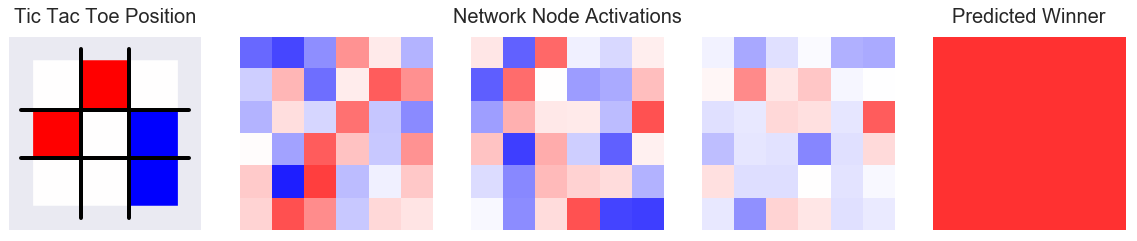
\includegraphics[width=1. \textwidth]{network_weights}
\end{figure}
\end{frame}

\section{Temporal Difference Learning}
\subsection{}
\begin{frame}{Temporal Difference Learning}
\begin{itemize}
\item TD($\lambda$) Equation
\end{itemize}
\begin{equation*}
T_n = \phantom{\sum_{n=0}^{N_0} }(1-\lambda)\phantom{\lambda^n} V_n + \lambda^{\phantom{N_0}} r
\end{equation*}
\end{frame}

\begin{frame}{Temporal Difference Learning}
\begin{itemize}
\item TD($\lambda$) Equation
\end{itemize}
\begin{equation*}
T_n = \sum_{n=0}^{N_0} (1-\lambda)\lambda^n V_n + \lambda^{N_0} r
\end{equation*}
\end{frame}
\section{Results}
\subsection{}

\begin{frame}
\begin{figure}
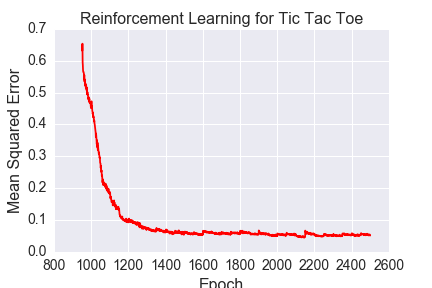
\includegraphics[width=1 \textwidth]{reinforcement_ttt}
\end{figure}
\end{frame}

\begin{frame}
\begin{figure}
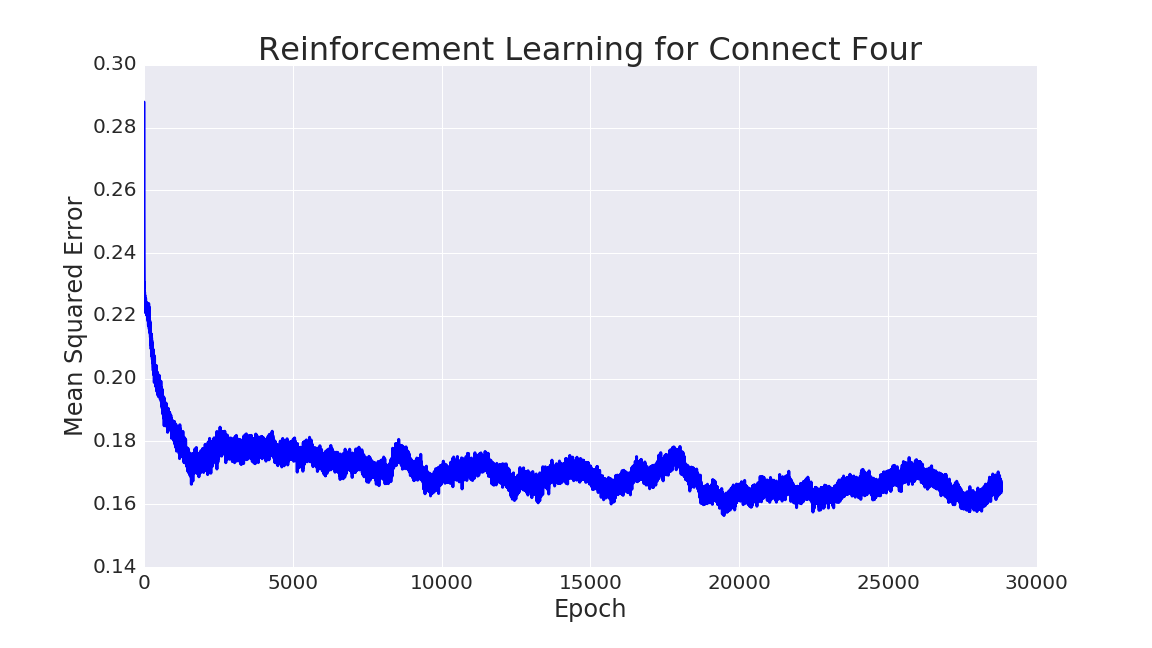
\includegraphics[width=1 \textwidth]{reinforcement_c4}
\end{figure}
\end{frame}

\begin{frame}
\begin{figure}
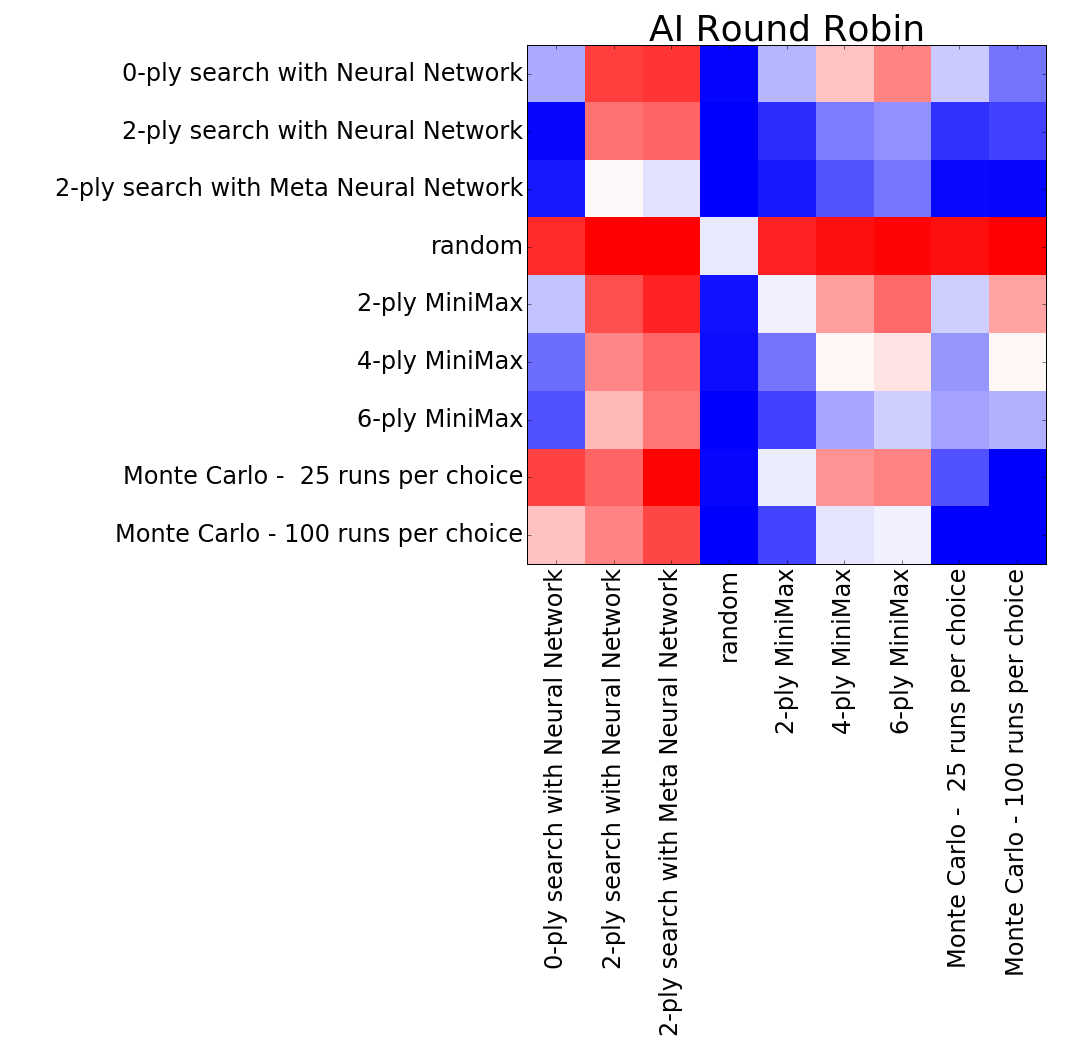
\includegraphics[width=0.70 \textwidth]{round_robin}
\end{figure}
\end{frame}

\begin{frame}
\begin{figure}
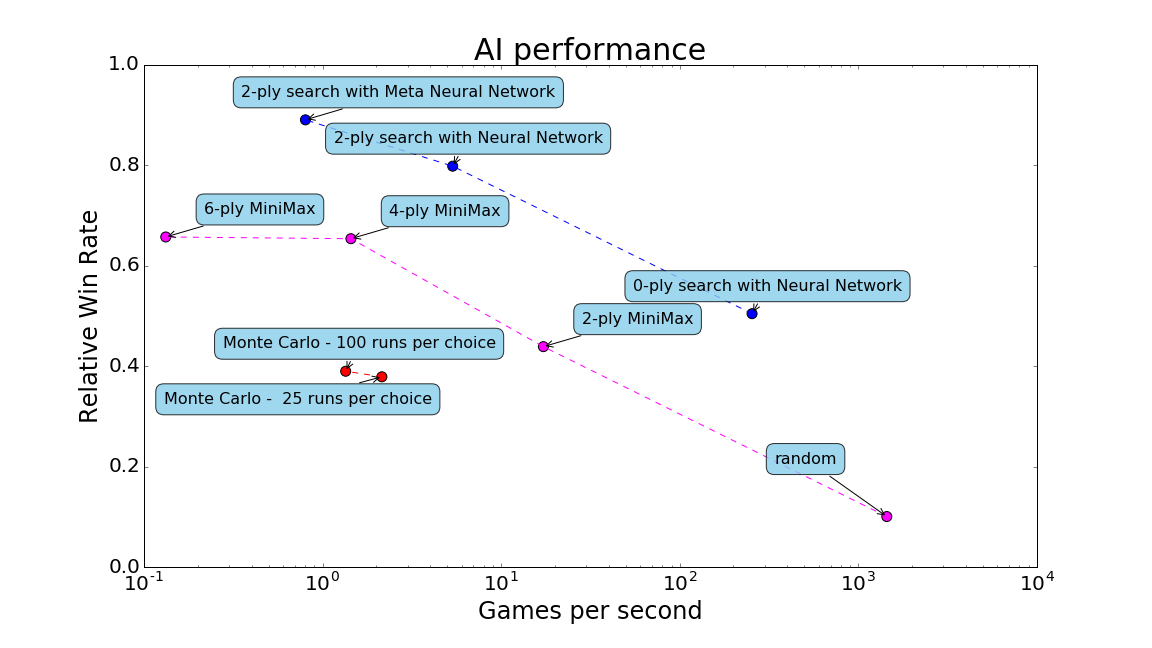
\includegraphics[width=1.0 \textwidth]{performance}
\end{figure}
\end{frame}
\section{Future Directions}
\subsection{}
\begin{frame}[c]{Future Directions}\centering
\begin{itemize}
\item Apply to more games
\begin{itemize}
\item chess, hex, backgammon, go, video games, etc.
\end{itemize}
\item Route finding app
\item Traffic prediction analysis
\item Control (robots, self-driving cars, etc.)
\item Prediction (stock prices, sports betting, etc.)
\item Acquire large data sets and compare with supervised learning
\end{itemize}
\end{frame}

\end{document}